% !TEX root = ../Report.tex

\subsection{Setup}

Python 3.6 or over can be chosen to design this solution. NiBabel package was used to deal with specificity of medical images. TensorFlow and Keras are additional libraries required to build training models and calculate metrics.
- slicer

\subsection{Training processes}
graph loss on training evaluation (dice loss, bce dice loss, batch size (correlates to gpu), epochs, steps per epoch, optimizer)

\begin{figure}[h!]
	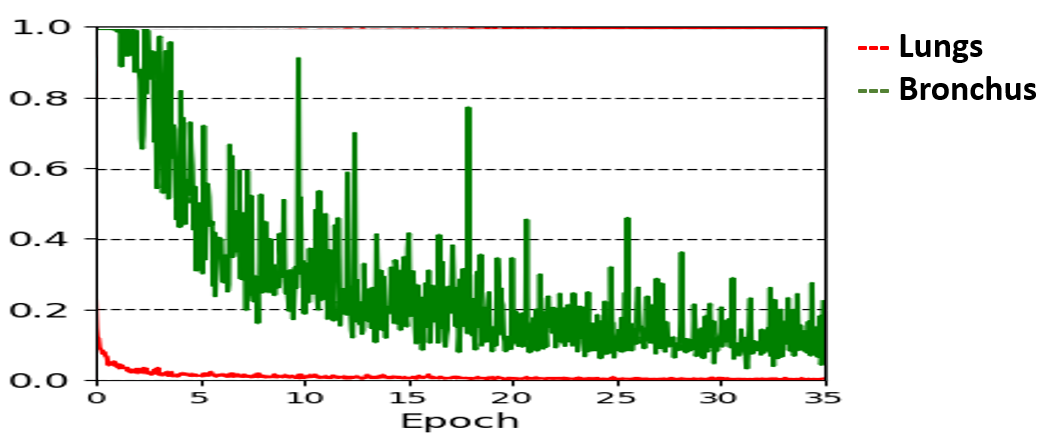
\includegraphics[width=0.49\textwidth, angle=0]{files/deepmedictrain.png}
	\caption{Training process of the DeepMedic architecture. The loss function (BCE) on the training data is shown for the lungs (red) and for the bronchus (green)}
	\label{train_deepmedic}
\end{figure}


\begin{figure}[h!]
	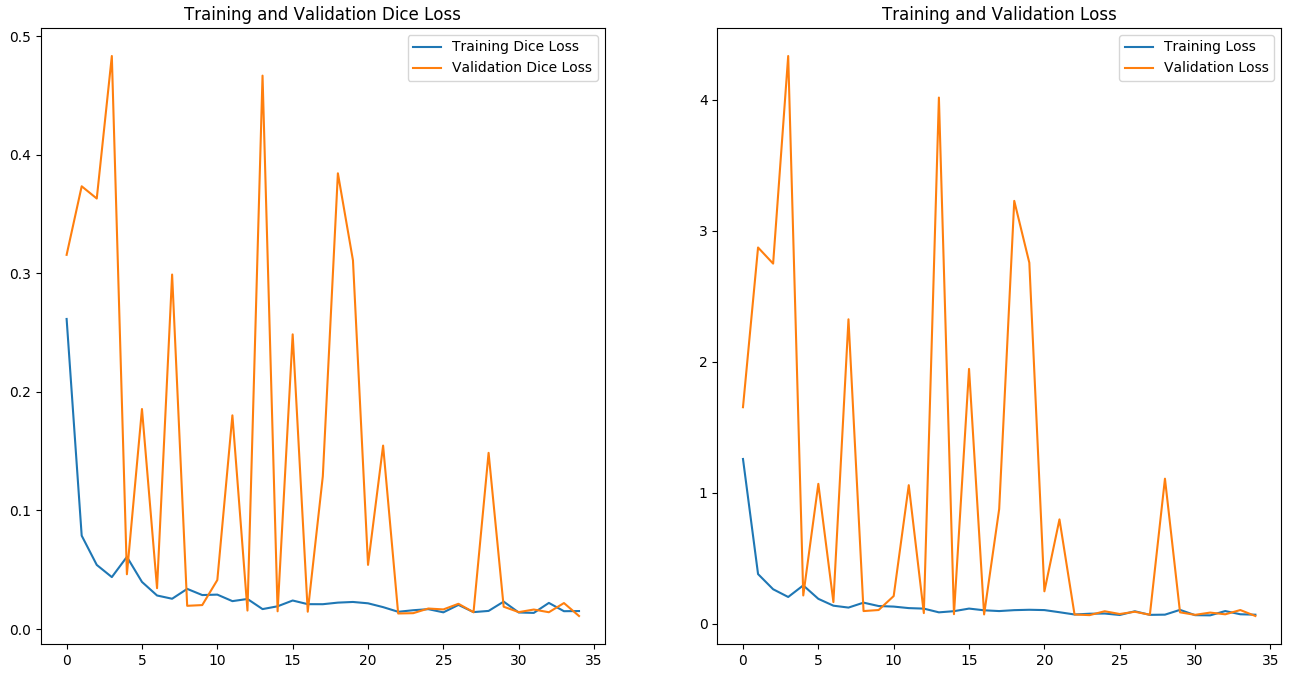
\includegraphics[width=0.49\textwidth, angle=0]{files/jpgunettrain.png}
	\caption{Training process of the U-Net architecture. The dice loss on the training and validation data is shown on the left. The actual loss function ($BCE + dice loss$) is shown on the right.}
	\label{train_unet}
\end{figure}

\begin{figure}[h!]
	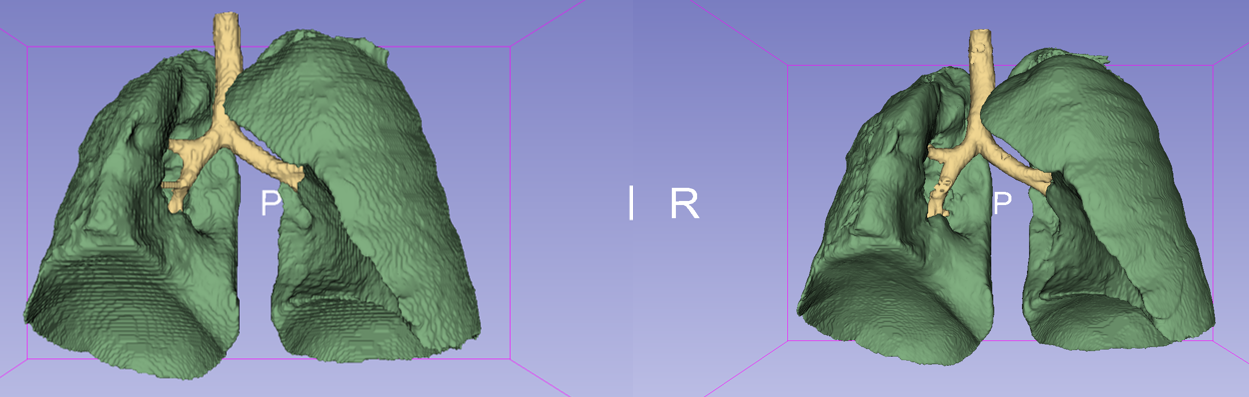
\includegraphics[width=0.49\textwidth, angle=0]{files/preddeepmedic.png}
	\caption{Example prediction of the DeepMedic architecture on one CT scan. The original label map for training is displayed on the left while the prediction of the network is shown on the right.}
	\label{pred_deepmedic}
\end{figure}

\begin{figure}[h!]
	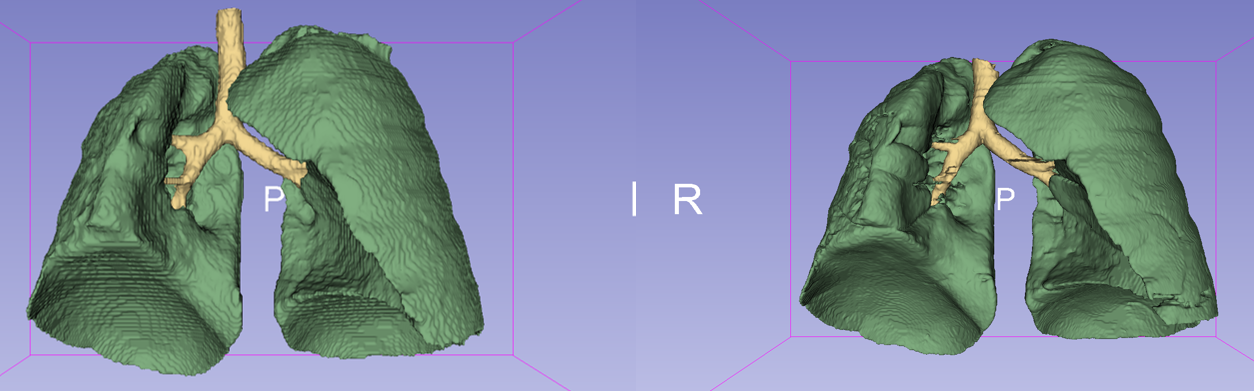
\includegraphics[width=0.49\textwidth, angle=0]{files/predunet.png}
	\caption{Example prediction of the DeepMedic architecture on one CT scan. The original label map for training is displayed on the left while the prediction of the network is shown on the right.}
	\label{pred_unet}
\end{figure}


\subsection{Evaluation of the two architectures}


comparison of unet and deepmedic

explain high hausdorff and how to reduce it


\begin{table}[h!]
	\centering
	\setlength{\tabcolsep}{10pt}
	\renewcommand{\arraystretch}{1.5}
	\begin{tabular}{c c c c}
		\hline 
		Architecture & Dice & Hausdorff & Mean \\
		& Coefficient & distance (mm) & Distance (mm) \\ 
		\hline 
		DeepMedic & 0.968 & 119.50 & 1.45 \\ 
		U-Net & 0.976 & 103.21 & 0.33 \\ 
		\hline
		\newline 
	\end{tabular}
	\caption{Dice Loss, Hausdorff distance and mean distance (on lungs and bronchus) averaged over 20 evaluation CT scans for the DeepMedic and the U-Net architecture.}
	\label{table_result}
\end{table}
